\section{SemantOS}
\label{sec:semantos}

\noindent SemantOS is an end-to-end semantic reasoning framework that transforms kernel parameter tuning from a static manual process into a sustained, explainable, verifiable control loop. Figure~\ref{fig:architecture} shows the architecture, organized around four design principles: \emph{context-aware}, \emph{knowledge-centric reasoning}, \emph{safety enforcement}, and \emph{continuous adaptation}.


\subsection{Design}
\label{sec:design}

\begin{figure}[t]
 \centering
 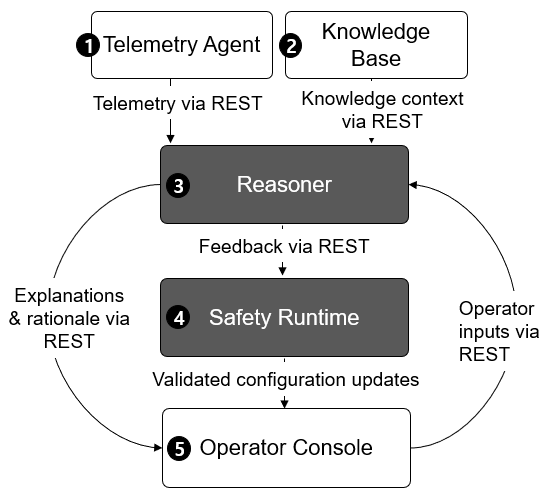
\includegraphics[width=0.64\linewidth]{figures/architecture.png}
 \caption{\textbf{SemantOS Control Loop Architecture.} The \emph{Telemetry Agent} collects kernel signals, the \emph{Knowledge Base} tracks typed inter-knob dependencies, the \emph{Reasoner} synthesizes \texttt{tuning-recommendations} grounded in retrieved graph evidence, and the \emph{Safety Runtime} validates and stages each update. Explanations, provenance, and rollback controls are surfaced to the operator through the \emph{Operator Console}.}
 
 \label{fig:architecture}
 \vspace{0.5pt}
\end{figure}

%=============================================
\scriptsize
\setlength{\tabcolsep}{5pt}
\renewcommand{\arraystretch}{0.95}
\begin{table}[t]
\centering
\begin{threeparttable}
\caption{\textbf{SOTA vs.\ SemantOS (aggregated).} Lower is better ($\downarrow$); operator time reduction higher is better ($\uparrow$). SemantOS values are means over 10 runs with 95\% CI half-widths.}
\label{tab:sota-compare}
\scriptsize
% Note: \resizebox is incompatible with threeparttable's width measurement
% (it makes the tabular invisible to the notes layout). We instead fit the
% table naturally by (a) tight \tabcolsep, and (b) dropping the redundant
% "up to" prefix on the SemantOS row -- already covered by the caption.
\setlength{\tabcolsep}{3pt}
\begin{tabular}{lcccc}
\toprule
\textbf{Method} & \textbf{Med.\ Lat.\,$\downarrow$} & \textbf{P95\,$\downarrow$} & \textbf{Anomaly\,$\downarrow$} & \textbf{Op.\ Time\,$\uparrow$} \\
\midrule
Expert profile           & --        & --        & --        & --        \\
AdaptiveKernel$^\dagger$ & 10--15\%  & 12--18\%  & 15--22\%  & 30--50\%  \\
OS-R1$^\dagger$          & 12--18\%  & 15--20\%  & 18--24\%  & 40--60\%  \\
BO/RL                    & 15--22\%  & 18--24\%  & 20--26\%  & 50--65\%  \\
\textbf{SemantOS}        & \textbf{23\,$\pm$\,1.4\%} & \textbf{28\,$\pm$\,1.7\%} & \textbf{31\,$\pm$\,2.1\%} & \textbf{85--92\%} \\
\bottomrule
\end{tabular}
\vspace{0.5pt}
\begin{tablenotes}
\footnotesize
\item \emph{$^\dagger$ Literature-reported ranges; setups differ.}
\item \emph{* Expert profile serves as the human reference baseline; improvements relative to itself are not applicable and therefore marked as ``--''.}
\end{tablenotes}
\end{threeparttable}
\end{table}
\normalsize
%========================================================


\begin{table}[t]
\centering
\setlength{\tabcolsep}{4pt}
\caption{\textbf{KB/RAG, Dependency-Graph, and Safety Ablation.} Median end-to-end latency
(ms; lower is better) and anomaly rate (\%; lower is better), reported under two regimes: \emph{stationary} workloads and \emph{drifting} workloads (where the workload mix shifts every 30\,minutes). The \emph{w/o Dep-Graph} variant tunes knobs independently (typed inter-knob edges removed), isolating the contribution of graph-grounded joint reasoning. Values are means over 10 runs with 95\% CI half-widths.}
\label{tab:ablation_kb_safety}
\scriptsize
% Wrap tabular in \resizebox so it never exceeds the AAAI single-column width.
\resizebox{\columnwidth}{!}{%
\begin{tabular}{lcccc}
\toprule
 & \multicolumn{2}{c}{\textbf{Latency (ms)}} & \multicolumn{2}{c}{\textbf{Anomaly Rate (\%)}} \\
\cmidrule(lr){2-3}\cmidrule(lr){4-5}
\textbf{Variant} & \textbf{Stationary} & \textbf{Drift} & \textbf{Stationary} & \textbf{Drift} \\
\midrule
Full SemantOS (KB+RAG+Safety) & 19.5\,$\pm$\,0.4 & 19.6\,$\pm$\,0.5 & 2.4\,$\pm$\,0.3 & 2.5\,$\pm$\,0.3 \\
\,\,w/o Dep-Graph (knobs indep.) & 21.4\,$\pm$\,0.5 & 21.6\,$\pm$\,0.6 & 4.1\,$\pm$\,0.4 & 4.4\,$\pm$\,0.5 \\
KB + Safety (w/o RAG)         & 21.2\,$\pm$\,0.5 & 21.3\,$\pm$\,0.6 & 3.6\,$\pm$\,0.4 & 3.8\,$\pm$\,0.4 \\
KB + RAG (w/o Safety)         & 19.8\,$\pm$\,0.4 & 20.0\,$\pm$\,0.5 & 4.9\,$\pm$\,0.5 & 5.2\,$\pm$\,0.6 \\
KB only                       & 22.6\,$\pm$\,0.6 & 22.7\,$\pm$\,0.7 & 7.1\,$\pm$\,0.7 & 7.6\,$\pm$\,0.8 \\
\bottomrule
\end{tabular}%
}
\vspace{0.5\baselineskip}
\end{table}



%======================================================
% NOTE: Runtime-footprint table moved to the technical supplement to keep the
% main paper within 7 pages under AAAI-compliant (default) float spacing.
% Its figures are stated inline in Implementation and Evaluation.
%======================================================


\paragraph{Design Goals.} We capture kernel signals, encode domain knowledge, emit explainable guarded updates, and preserve SLOs via staged enforcement. Guardrails are declarative policies (SLO targets, invariants, per-knob bounds) enforced by the runtime regardless of model output.

\paragraph{Components.}
The loop has five core components, each a service directory in the artifact. The \textbf{\ding{182} Telemetry Agent} collects eBPF and user-space metrics every 5\,s; the \textbf{\ding{183} Knowledge Base} stores tunable metadata, the typed dependency graph, and historical traces, autonomously refining relationships via telemetry and decayed weights. The \textbf{\ding{184} Reasoner} uses retrieval-augmented prompts to emit \textsc{knob}, \textsc{value}, \textsc{rationale}, and \textsc{uncertainty}. The \textbf{\ding{185} Safety Runtime} enforces staged rollout, monitors SLOs, and triggers veto/rollback. The \textbf{\ding{186} Operator Console} provides an explanatory interface and auditability. Algorithm~\ref{alg:control-loop} summarizes the loop.

\begin{algorithm}[t]
\caption{SemantOS Control Loop}
\label{alg:control-loop}
\begin{algorithmic}[1]
\REQUIRE Knowledge base $G$, calibration set $\mathcal{D}_{\mathrm{cal}}$, SLO bounds $\{\ell_i\}$, threshold $\tau$, decay $\gamma$
\WHILE{system is running}
  \STATE $T_t \leftarrow \textsc{TelemetryAgent.snapshot}()$ \hfill\textit{// eBPF + userspace}
  \STATE $E_t \leftarrow \textsc{KB.retrieve}(T_t, G)$ \hfill\textit{// typed graph + FAISS}
  \STATE $(\textit{knob},\textit{val},\textit{rat},u) \leftarrow \textsc{Reasoner.LLM}(T_t, E_t)$
  \IF{$u \ge \tau$ \OR $\textsc{SLOGuard}(T_t,\textit{knob},\textit{val})$ fires}
    \STATE \textbf{continue} \hfill\textit{// veto: emit no-op}
  \ENDIF
  \FOR{$\textit{stage}\in\{\text{canary},\text{ramp},\text{full}\}$}
    \STATE Apply $(\textit{knob},\textit{val})$ at $\textit{stage}$ traffic share
    \IF{regression detected on $\{\ell_i\}$}
      \STATE \textsc{Rollback}; \textsc{KB.log}($\textit{OptimizationTrace}$); \textbf{break}
    \ENDIF
  \ENDFOR
  \STATE \textsc{KB.update}$(T_t,\textit{outcome},\gamma)$ \hfill\textit{// ADWIN drift}
  \STATE Periodically refresh $\tau$ from $\mathcal{D}_{\mathrm{cal}}$ \hfill\textit{// recalibration}
\ENDWHILE
\end{algorithmic}
\end{algorithm}

\paragraph{Knowledge-Centric Decision Loop and Safety Argument.}
Each decision fuses telemetry with retrieved KB context; the uncertainty $u$ gates whether an action is approved, delayed, or rolled back, and every update carries a rationale over telemetry, KB evidence, and audit trail. With canary$\to$ramp$\to$full rollout and continuous SLO monitoring, unsafe recommendations are rolled back before system-wide impact---formalized as expected-cost and drift-recovery guarantees in Theorem~\ref{thm:pac-cost} and Proposition~\ref{prop:recal}. In practice this preserves no-worse-than-default behavior in expectation under observed drift (Table~\ref{tab:ablation_kb_safety}).



\subsection{Semantic Reasoning}
\label{sec:semantic}
SemantOS's semantic inference layer fuses structured domain knowledge, past experience, and LLM inference in one safe decision loop. The hybrid KB combines tunable metadata, a typed dependency graph, and a FAISS (Facebook AI Similarity Search)-powered trace store.

\noindent\textbf{Typed dependency graph.} Each node is a tunable annotated with its type, admissible range, unit, and subsystem (scheduler, memory, I/O, IRQ, NUMA). Edges are \emph{typed and signed}: \textsc{depends-on} (a knob's safe range is conditioned on another's value), \textsc{conflicts-with} (joint change risks an SLO regression), and \textsc{synergizes-with} (joint change yields super-additive gains). Edges are \emph{induced offline} from the pairwise co-tuning sweeps of our empirical study (Motivation): for a knob pair $(a,b)$ we estimate the interaction as the deviation of the joint effect from the additive single-knob effects on the target metric; a positive/negative deviation exceeding a bootstrap significance threshold yields a \textsc{synergizes-with}/\textsc{conflicts-with} edge, and a range-conditioning relation (detected when $a$'s safe interval shifts with $b$) yields \textsc{depends-on}. Each edge then carries a weight that is \emph{decayed online} by $\gamma^t$ and refreshed from deployment telemetry, so stale couplings fade. Seed edges and the induction script are released in the artifact. This typing is what lets SemantOS reason about \emph{inter-knob} effects that black-box tuners treat as independent dimensions (cf.\ Observation~2, Fig.~\ref{fig:pairwise}).

\noindent\textbf{Graph-grounded joint reasoning.} On each invoked snapshot a composite query runs: a graph query expands the candidate knob's typed neighborhood (its \textsc{conflicts-with}/\textsc{synergizes-with} edges) into structural constraints, while vector search returns nearest-neighbor traces (prior configurations, metrics, notes) as evidence. Serialized into the prompt, this forces the Reasoner to \emph{co-tune} along synergistic edges and \emph{justify against} conflicting neighbors rather than proposing a knob in isolation, so each recommendation carries provenance to specific KB edges and traces. Using this evidence the Reasoner emits a rationale plus a calibrated uncertainty $u\!\in\![0,1]$ consumed by the safety runtime.

\subsection{Theoretical Guarantees}
\label{subsec:theorem}

\noindent\textbf{What ``unsafe'' means (calibration ground truth).} An applied action is labeled \emph{unsafe} \emph{post hoc} if, within its staged-rollout window, it violates any declarative SLO guard (a per-metric bound $\ell_i$, e.g., a P95-latency or anomaly-rate ceiling) and triggers a rollback. The calibration set $\mathcal{D}_{\mathrm{cal}}$ is the held-out log of past (telemetry, KB-evidence, action, uncertainty $u$, outcome-label) tuples collected under this rule; because the outcome label is derived from the same SLO guards the runtime enforces, no manual annotation is required and the label is reproducible from the released logs. The score used for calibration is the recommendation's uncertainty $u\in[0,1]$.

We assume \emph{exchangeable} coverage of $\mathcal{D}_{\mathrm{cal}}$; if drift violates this, we recalibrate on a sliding window to maintain error control. Conformal calibration on $\mathcal{D}_{\mathrm{cal}}$ yields a threshold $\tau$ such that
$\Pr[\text{unsafe}\mid u<\tau]\le\alpha$, ensuring $1-\alpha$ marginal coverage (cf.~\citeauthor{Jeary2024NeurIPS}~\citeyear{Jeary2024NeurIPS}; \citeauthor{Correia2024NeurIPS}~\citeyear{Correia2024NeurIPS}).

\vspace{0.5\baselineskip}
\begin{theorem}[Expected-Cost Decomposition]\label{thm:pac-cost}
Let recommendations be drawn from a (possibly time-varying) distribution that is exchangeable within each calibration window. Let $c_{\mathrm{FN}},c_{\mathrm{FP}}\!\ge\!0$ be the costs of, respectively, accepting an unsafe action and vetoing a safe action, $\pi\!=\!\Pr[\text{unsafe}]$ the base rate, and $\lambda\!\ge\!0$ the SLO penalty weight. Under the SemantOS safety policy (veto if $u\ge\tau$ \emph{or} an SLO guard fires; otherwise apply via canary~$\rightarrow$~ramp~$\rightarrow$~full staged rollout), the expected per-decision cost $C$ (defined as the sum of the three cost components below) satisfies
\begin{equation}\label{eq:cost-bound}
\mathbb{E}[C] \;\le\; \underbrace{c_{\mathrm{FN}}\,\pi\,\alpha}_{\text{Safety Risk}}
\;+\; \underbrace{c_{\mathrm{FP}}\,(1-\pi)\,\beta_{\mathrm{FP}}}_{\text{Efficiency Loss}}
\;+\; \underbrace{\lambda\,\mathbb{E}[\Delta\mathrm{SLO}]}_{\text{Perf. Degradation}},
\end{equation}
where $\alpha$ is the conformal miss rate for unsafe actions, $\beta_{\mathrm{FP}}\!=\!\Pr[\mathrm{safe}\mid u\!\ge\!\tau]$ denotes the false-positive (over-veto) probability, and $\Delta\mathrm{SLO}$ is the SLO deviation incurred during the canary/ramp window before rollback.
\end{theorem}

\noindent\textit{Proof sketch.} (i)~By the validity of split conformal prediction under exchangeable calibration, $\Pr[\text{unsafe}\wedge u<\tau]\!\le\!\pi\alpha$, so accepting a sample below $\tau$ contributes at most $c_{\mathrm{FN}}\pi\alpha$ in expectation. (ii)~Vetoing a safe sample (false positive) occurs with probability $(1\!-\!\pi)\beta_{\mathrm{FP}}$ and contributes $c_{\mathrm{FP}}(1\!-\!\pi)\beta_{\mathrm{FP}}$. (iii)~For accepted unsafe samples, staged rollout caps the worst-case traffic share exposed before the SLO guard triggers a rollback; bounding this exposure by $\Delta\mathrm{SLO}$ and applying the SLO penalty $\lambda$ yields the third term. Since $C$ is \emph{defined} as the sum of the three components, linearity of expectation---not any independence assumption---gives Eq.~\ref{eq:cost-bound}. Under sliding-window recalibration, $\alpha$ and $\beta_{\mathrm{FP}}$ remain valid after each refresh; the coverage-recovery guarantee is made precise in Proposition~\ref{prop:recal}.\hfill$\square$

\vspace{0.5\baselineskip}
We stress the modest scope of Eq.~\ref{eq:cost-bound}: it is a conformal \emph{risk-control decomposition}, not a PAC/sample-complexity bound. Its value is operational---it names the three levers ($\alpha$, $\beta_{\mathrm{FP}}$, $\Delta\mathrm{SLO}$) a deployment can tune and shows the safety term is controlled by the conformal miss rate $\alpha$. Its substantive content under non-stationarity is the recalibration guarantee we make explicit next, which is the property a deployment actually relies on.

\vspace{0.3\baselineskip}
\begin{proposition}[Recalibration coverage recovery under drift]\label{prop:recal}
Suppose a drift event changes the score distribution so that its total-variation distance from the active calibration distribution is at most $\varepsilon$. Under sliding-window recalibration with window size $m$, once the window has refilled with post-drift, within-window exchangeable scores, the realized unsafe-acceptance rate $\alpha'$ obeys
\[
\alpha' \;\le\; \alpha \;+\; \tfrac{1}{m+1} \;+\; \varepsilon ,
\]
and $\alpha' \to \alpha + \tfrac{1}{m+1}$ as the window fully refreshes ($\varepsilon\!\to\!0$). Hence the target coverage is restored up to the finite-sample slack $\tfrac{1}{m+1}$ after recalibration completes.
\end{proposition}

\noindent\textit{Proof sketch.} Within a refilled window the post-drift scores are exchangeable, so split-conformal validity gives a miss rate at most $\lceil(1-\alpha)(m+1)\rceil/(m+1)\le\alpha+\tfrac{1}{m+1}$. During the transient before the window refills, the score law differs from the calibration law by at most $\varepsilon$ in total variation, which can inflate the acceptance rate by at most $\varepsilon$ (the maximal event-probability gap under a TV constraint). Summing the two contributions yields the bound; the transient term vanishes as old samples age out. Larger $m$ tightens the slack but lengthens the transient---a trade-off we set empirically ($m$ giving a $\le\!1\%$ slack) and validate in the 30-day drift study.\hfill$\square$

\vspace{0.3\baselineskip}
Here, $\beta_{\mathrm{FP}}$ represents the probability of a high-uncertainty action being safe, modulating false-positive costs by penalizing interventions whose uncertainty-adjusted risk exceeds the calibrated regime. We use the notation $\beta_{\mathrm{FP}}$ to avoid confusion with the unrelated DPO temperature $\beta_{\mathrm{DPO}}$ used in training (see \emph{Implementation}).

\paragraph{Safety Runtime Feedback.}
The \texttt{SafetyRuntime} uses $u$ with real-time SLO guards to accept, delay, or veto; rollbacks emit an \texttt{OptimizationTrace} to the KB for continual refinement and re-calibration. The end-to-end ablation of KB/RAG and safety is deferred to the Evaluation (Table~\ref{tab:ablation_kb_safety}).

\subsection{Implementation}
\label{sec:implementation}

We implement SemantOS as a modular, Representational State Transfer (REST)-based distributed system of five containerized services that communicate via typed messages defined in \texttt{proto/semantos-control.v1.yaml}; an anonymized artifact reproduces the prototype end-to-end via \texttt{Makefile} targets.

\noindent\textbf{Services.}
\texttt{telemetry-agent/} (Python/C, eBPF) samples every 5\,s and exports \texttt{TelemetrySnapshots} ($<\!1\%$ CPU). \texttt{kb-service/} stores tunable metadata, the typed dependency graph, and traces (\texttt{RetrieveContext}, \texttt{LogOutcome}). \texttt{reasoner/} serves \texttt{/get\_recommendations} (returning \texttt{knob\_name}, \texttt{proposed\_value}, \texttt{rationale}, \texttt{expected\_impact}, $u\!\in\![0,1]$), \texttt{/apply}, and \texttt{/log\_outcome}. \texttt{safety-runtime/} enforces staged rollout (canary$\to$ramp$\to$full) and rolls back when $u\!\ge\!\tau$ or guardrails fire. The optional \texttt{operator-console/} (FastAPI) surfaces telemetry, evidence, and suggestions with override/rollback controls.

\noindent\textbf{LLM training pipeline (Reasoner).}
A 13B decoder-only model (LLaMA-3.1-13B; chosen as the largest model that meets our single-A100 side-car budget) is fine-tuned in five stages: (1)~\emph{data} from public kernel documentation and anonymized context--action--outcome traces from our simulator. To prevent train/test contamination, the six evaluation workloads and the three evaluation server classes are \emph{held out} from all fine-tuning and simulator-trace generation; only disjoint workload--hardware pairs feed training. Then: (2)~\emph{annotation} of (telemetry, KB evidence) tuples mapped to (recommendation, rationale, impact, uncertainty hint); (3)~\emph{SFT} (context $L\!=\!4$--$8$K, AdamW, cosine decay, label smoothing 0.05, early stopping; effective batch 256, $\mathrm{lr}\!=\!2\!\times\!10^{-5}$, warmup 2\%, weight decay 0.1, grad-clip 1.0); (4)~optional \emph{DPO}-style pairwise alignment ($\beta_{\mathrm{DPO}}\!=\!0.1$, distinct from the calibration-side $\beta_{\mathrm{FP}}$ in Theorem~\ref{thm:pac-cost}) toward provenance-grounded, low-anomaly explanations; and (5)~\emph{hallucination mitigation} via retrieval grounding, constrained decoding (deny-list/out-of-range), self-consistency voting, and provenance checks; low-confidence ($u\!\ge\!\tau$) or ungrounded outputs are vetoed. Full configuration is released in the artifact.

\vspace{0.6\baselineskip}
\noindent
Three core JSON endpoints (\texttt{POST~/get\_recommendations}, \texttt{/apply}, \texttt{/log\_outcome}) close the telemetry$\to$recommendation$\to$deployment$\to$feedback loop. The KB is updated via exponential decay on dependency weights ($\gamma^t$) and ADWIN drift detection. On the fast path ($\approx\!94\%$ of snapshots) the system decides within 10\,ms at $<\!3\%$ CPU and $<\!300$\,MB (full per-path footprint in the supplement); the 13B Reasoner runs asynchronously on a GPU side-car for the $\approx\!6\%$ of snapshots exceeding a guarded deviation threshold, so its decode latency never blocks enforcement. All decisions and rationales are immutably logged.


